\newacronym{prbs}{PRBS}{\textit{Pseudo-Random Binary Signal}}
\newacronym{arma}{ARMA}{\textit{Auto-Regressive Moving Average}}
\newacronym{gbn}{GBN}{\textit{Generalized Binary Noise}}
\newacronym{ar}{AR}{Modelo autorregressivo}
\newacronym{arx}{ARX}{Modelo autorregressivo com entrada exógena}
\newacronym{armax}{ARMAX}{Modelo autorregressivo com média móvel e entrada exógena}
\newacronym{aic}{AIC}{Critério de informação de Akaike}
\newacronym{oe}{OE}{\textit{Output-Error}}
\newacronym{bj}{BJ}{Box-Jenkins}
\newacronym{nlarx}{NLARX}{ARX não-linear}

\chapter{Metodologia}
\label{ch:metodologia}

% =====================================================================================================
% ============================================= Section ===============================================
% =====================================================================================================
\section{Modelagem experimental}
\label{sec:modelagem_experimental}

Segundo \citeonline{Gevers2006} a teoria de identificação de sistemas data da década de 60 e as duas
principais técnicas utilizadas na identificação de sistemas atualmente (método de identificação por
subespaço de estados e método do erro de predição) tiveram suas bases estruturadas com os trabalhos
de \apudonline{Ho1966}{Gevers2006} e de \apudonline{Astrom1965}{Gevers2006}.

De acordo com \apudonline{Dunia2008}{Pracek2012} a identificação do sistema permite que simulações
sejam desenvolvidas de modo a garantir um melhor desempenho dos sistemas de controle projetados.

As etapas para a identificação de um sistema, segundo \citeonline{Aguirre2015} são:
\begin{itemize}
    \item Testes dinâmicos e coleta de dados
    \item Escolha da representação matemática a ser utilizada
    \item Determinação da estrutura do modelos
    \item Estimação de parâmetros
    \item Validação do modelo
\end{itemize}

As seções a seguir detalham cada uma dessas etapas.

% .....................................................................................................
% ............................................ Subsection .............................................
% .....................................................................................................
\subsection{Testes dinâmicos e coleta de dados}
\label{subsec:testes_dinamicos_e_coleta_de_dados}

Esta etapa abrange os procedimentos necessários para geração do conjunto de dados que serão utilizados
para a identificação do sistema. Algumas das atividades realizadas nessa etapa são: escolha das variáveis,
definição dos sinais de excitação, definição do período de amostragem e execução de testes.
\cite{Aguirre2015}

% -----------------------------------------------------------------------------------------------------
% ------------------------------------------- Subsubsection -------------------------------------------
% -----------------------------------------------------------------------------------------------------
\subsubsection{Período de amostragem}
\label{subsubsec:periodo_de_amostragem}

Segundo o teorema de Shannon, descrito por \citeonline{Aguirre2015}, "um sinal que não contenha componentes
de frequência acima de $1/2T_s$ pode ser determinado unicamente a partir de amostras de tal sinal separadas
por $T_s$", sendo $T_s$ o período de amostragem ou, como também é chamado, tempo de amostragem.

Na prática, contudo, um período de amostragem apenas 2 vezes maior que a frequência de interesse, como exigido
pelo teorema de Shannon, nem sempre é suficiente. Normalmente então escolhe-se uma frequência de amostragem
entre 5 e 10 vezes maior do que a maior do que tal frequência desejada \cite{Aguirre2015}. Por outro lado, do
ponto de vista numérico, se o intervalo de amostragem for muito curto, a estimação de parâmetros também
poderá se tornar malcondicionada \cite{Aguirre2015}.

Para a identificação da maior frequência de interesse do sistema analisado, alguns ensaios foram realizados\footnote{
    Indicar scripts utilizados          % TODO Indicar scripts utilizados
}
excitando o Aquecedor 1 do \acrshort{tclabsp} em $50\%$ e aproximando a resposta em malha aberta dos
Sensores de Temperatura 1 e 2 para um sistema de primeira ordem, a fim de obter o valor do tempo de subida
($\tau$). Esse tempo de subida servirá de referência para o cálculo do período de amostragem.

\begin{figure}[h]
	\caption{Tempo de subida - Sensor de Temperatura 1}
	\begin{center}
		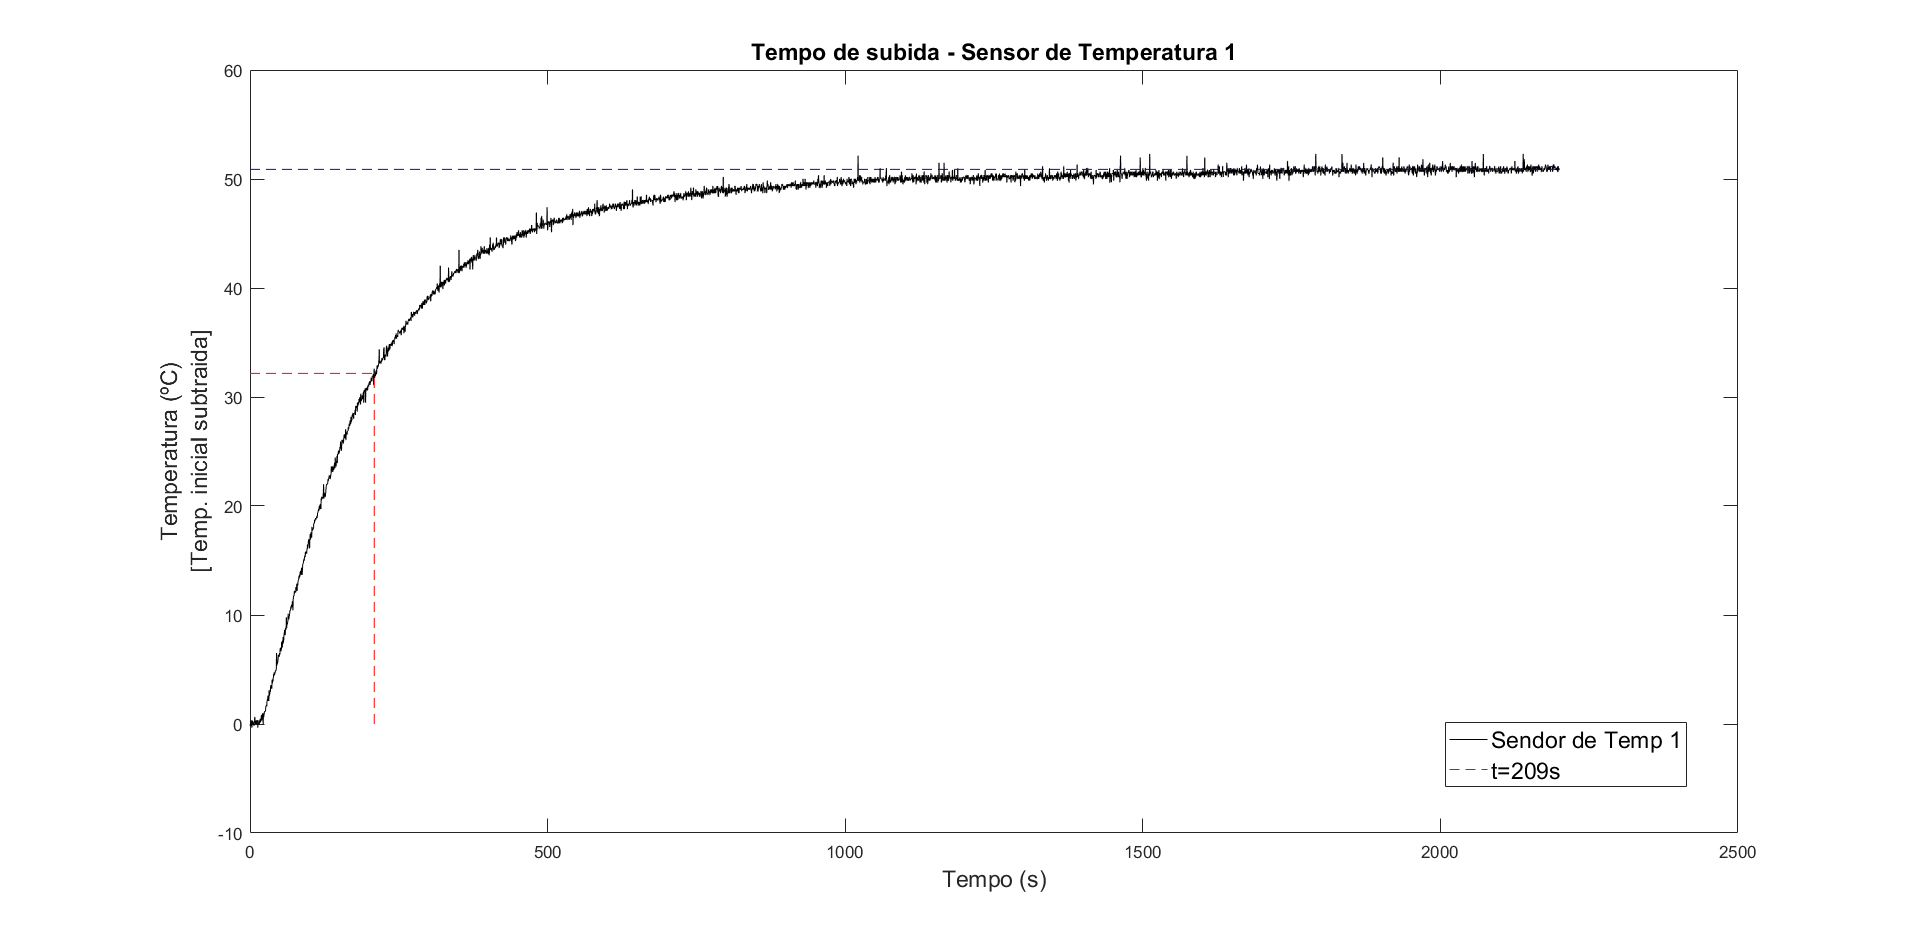
\includegraphics[width=0.95\textwidth]{./5_images/RiseTime-TempSensor1.png} 
		\label{fig:rise_time_sensor1}
	\end{center}
	\centering
	\makebox[\width]{Fonte: \citeonline{Prata2019}} 
\end{figure}

\begin{figure}[h]
	\caption{Tempo de subida - Sensor de Temperatura 1}
	\begin{center}
		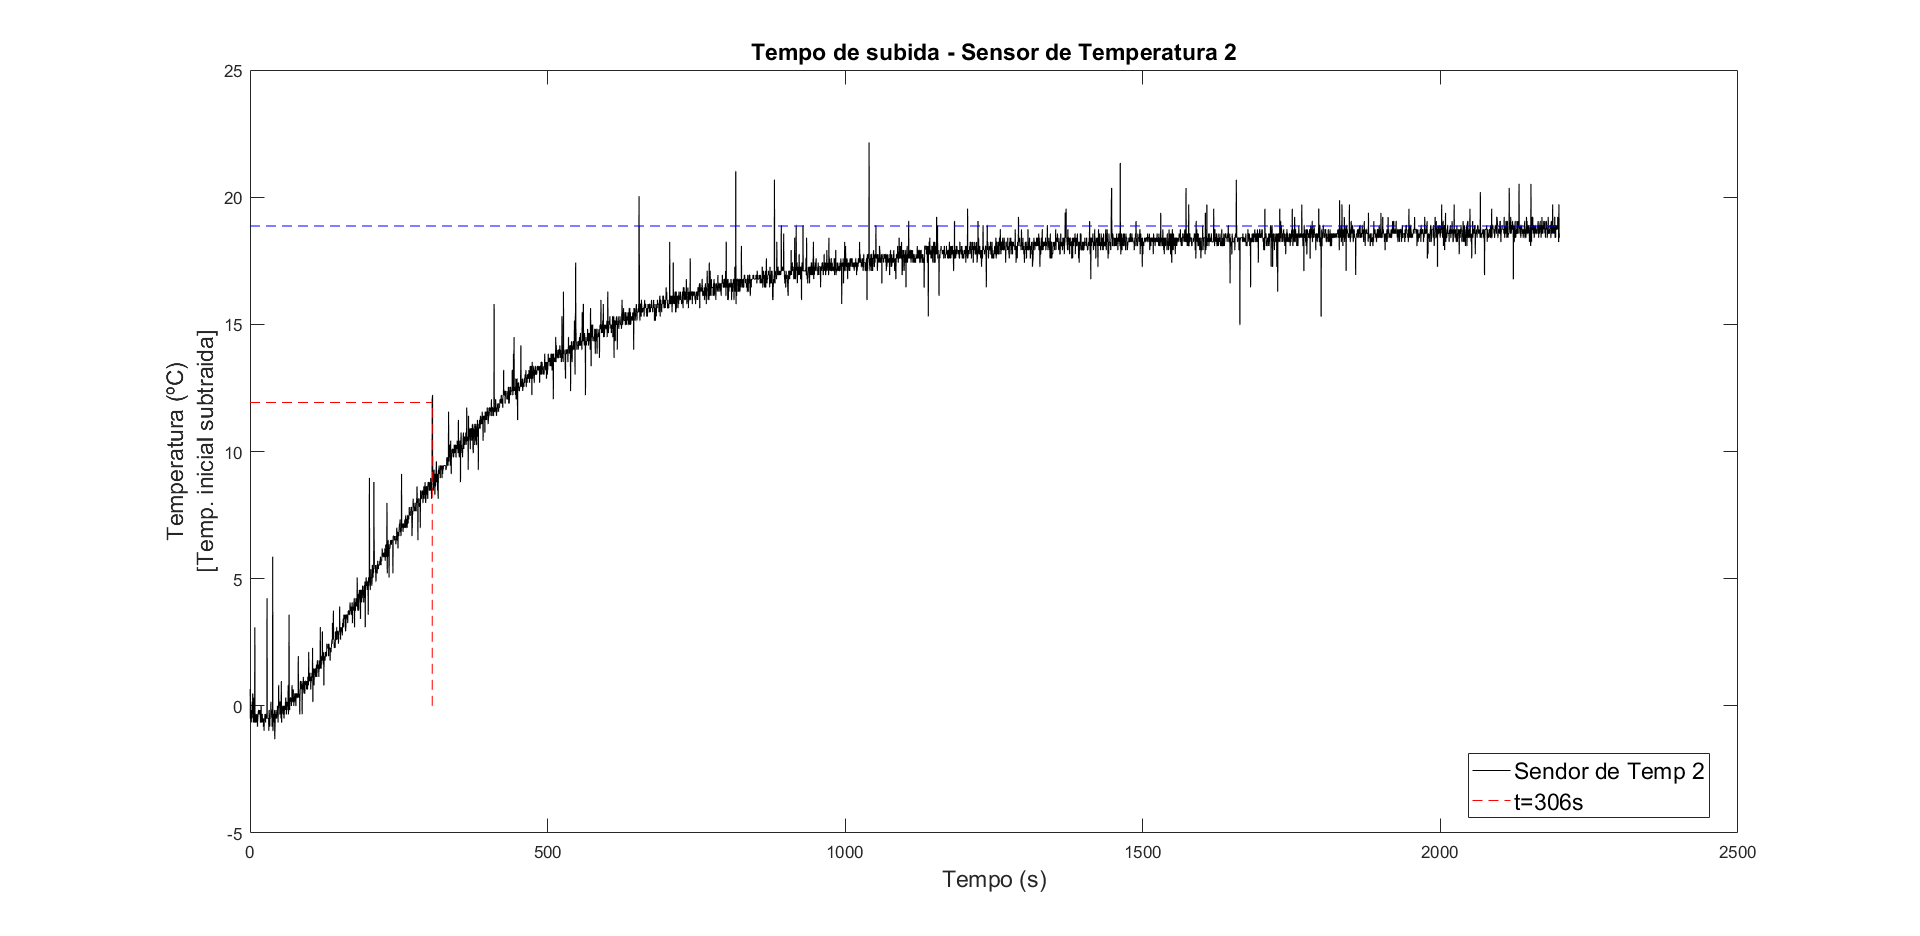
\includegraphics[width=0.95\textwidth]{./5_images/RiseTime-TempSensor2.png} 
		\label{fig:rise_time_sensor2}
	\end{center}
	\centering
	\makebox[\width]{Fonte: \citeonline{Prata2019}} 
\end{figure}

As \cref{fig:rise_time_sensor1,fig:rise_time_sensor2} mostram a resposta em malha aberta dos Sensores de
Temperatura 1 e 2, respectivamente, a uma entrada degrau no Aquecedor 1. Este ensaio foi realizado com
um período de amostragem de 0,5s, e com ele foi possível observar um tempo de subida $\tau_1 = 209s$ para
o Sensor 1 e $\tau_2 = 383s$ para o Sensor 2.
% TODO: Fazer mais ensaios com step 0 -> 50
% TODO: Recortar as imagens para remover bordas brancas

Seguindo a regra prática de \citeonline{Aguirre2015} onde $T_s$ deve ser entre 5 e 10 vezes maior que a
maior frequência desejada, então temos que $20.9s > T_s > 41.8s$.

Para os ensaios realizados neste trabalho, optou-se pela maior frequência de amostragem possível, como
mostrado na \cref{eq:sampling_time}.

\begin{equation}
	\label{eq:sampling_time}
	T_s = 20.9s
\end{equation}

Outra técnica também descrita por \citeonline{Aguirre2015} para a escolha da frequência de amostragem,
apesar de não ter sido escolhida, também foi testada e é descrita em maiores detalhes no
\cref{ch:sampling_time_using_autocorrelation}.

% -----------------------------------------------------------------------------------------------------
% ------------------------------------------- Subsubsection -------------------------------------------
% -----------------------------------------------------------------------------------------------------
\subsubsection{Sinais de excitação}
\label{subsubsec:sinais_de_excitacao}

% \acrshort{arma} - Média Móvel Auto-Regressiva (do inglês, \acrlong{arma})
A escolha dos sinais de entrada pode ter grande impacto nos dados coletados,
pois determinarão o ponto de operação do sistema e quais das suas características serão excitadas
durante o experimento \cite{Aguirre2015}.
Diversos tipos distintos de sinais podem ser utilizados. Entre os mais comuns destacam-se:
impulsivo; degrau; \acrshort{prbs} - Sinal Binário Pseudo-Aleatório (do inglês, \acrlong{prbs});
\acrshort{gbn} - Ruido Binário Generalizado (do inglês, \acrlong{gbn}); soma de senóides e etc \cite{Aguirre2015}.
Porém quando objetiva-se a identificação do sistema de onde os dados foram coletados, no geral
os métodos de identificação exigem que os sinais de entrada tenham um espectro de frequência
branco ou quase branco. Sinais aleatórios e pseudoaleatórios satisfazem essa condição \cite{Aguirre2015}.

Sinais \acrshort{prbs} são comumente usados na identificação de sistemas lineares, porém para sistemas
não-lineares tais sinais não são adequados, neste caso muitas vezes será desejável excitar o
sistema numa larga faixa de amplitudes a fim de poder observar suas características estáticas e dinâmicas
\cite{Aguirre2015}.

\begin{citacao}
    Características dinâmicas e estáticas que não forem excitadas não aparecerão nos dados. O que
    não estiver nos dados não pode ser identificado. Tal princípio é utilizado, por exemplo,
    quando um sistema é excitado em torno de um ponto de operação. Neste caso, como as não-linearidades
    não foram excitadas no teste, é possível, pelo menos em princípio, ajustar um modelo linear
    aos dados assim obtidos. \cite{Aguirre2015}
\end{citacao}

Segundo \citeonline{Aguirre2015} uma regra prática para a aplicação do sinal de excitação é,
tendo-se definido o tempo de amostragem (já discutido na \cref{subsubsec:periodo_de_amostragem}),
manter constante o valor escolhido aleatóriamente por um tempo, em torno de 3 a 5 intervalos de
amostragem.

Para a coleta dos sinais do \acrshort{tclabsp} foram aplicados tanto no Aquecedor 1 quanto no
Aquecedor 2 sinais de entrada aleatórios, mantidos constantes por um período de $3T_s$ a $5T_s$
(vide \cref{eq:sampling_time}). Contudo, antes dos sinais aleatórios serem aplicados aos
aquecedores, um sinal constante de $50\%$ foi aplicado a cada um deles por $1500s$ com o intuito
de estabilizá-los em um patamar onde as amplitudes dos sinais aleatórios aplicados tivessem
maior liberdade. A \cref{fig:simulink_coleta} mostra o modelo \textit{Simulink} utilizado para
a coleta dos dados e a \cref{fig:experiment_inputs} mostra os sinais de entrada aplicados nos
Aquecedores 1 e 2.

\begin{figure}[h]
	\caption{Modelo \textit{Simulink} para coleta de dados}
	\begin{center}
		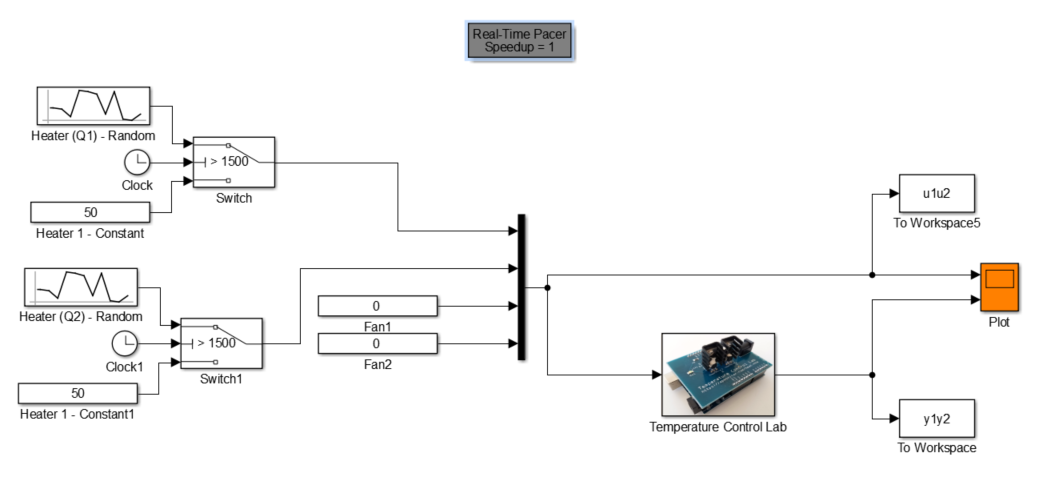
\includegraphics[width=0.85\textwidth]{./5_images/SimulinkColeta.png} 
		\label{fig:simulink_coleta}
	\end{center}
	\centering
	\makebox[\width]{Fonte: Autor} 
\end{figure}

\begin{figure}[h]
	\caption{Sinais de entrada nos Aquecedores 1 e 2}
	\begin{center}
		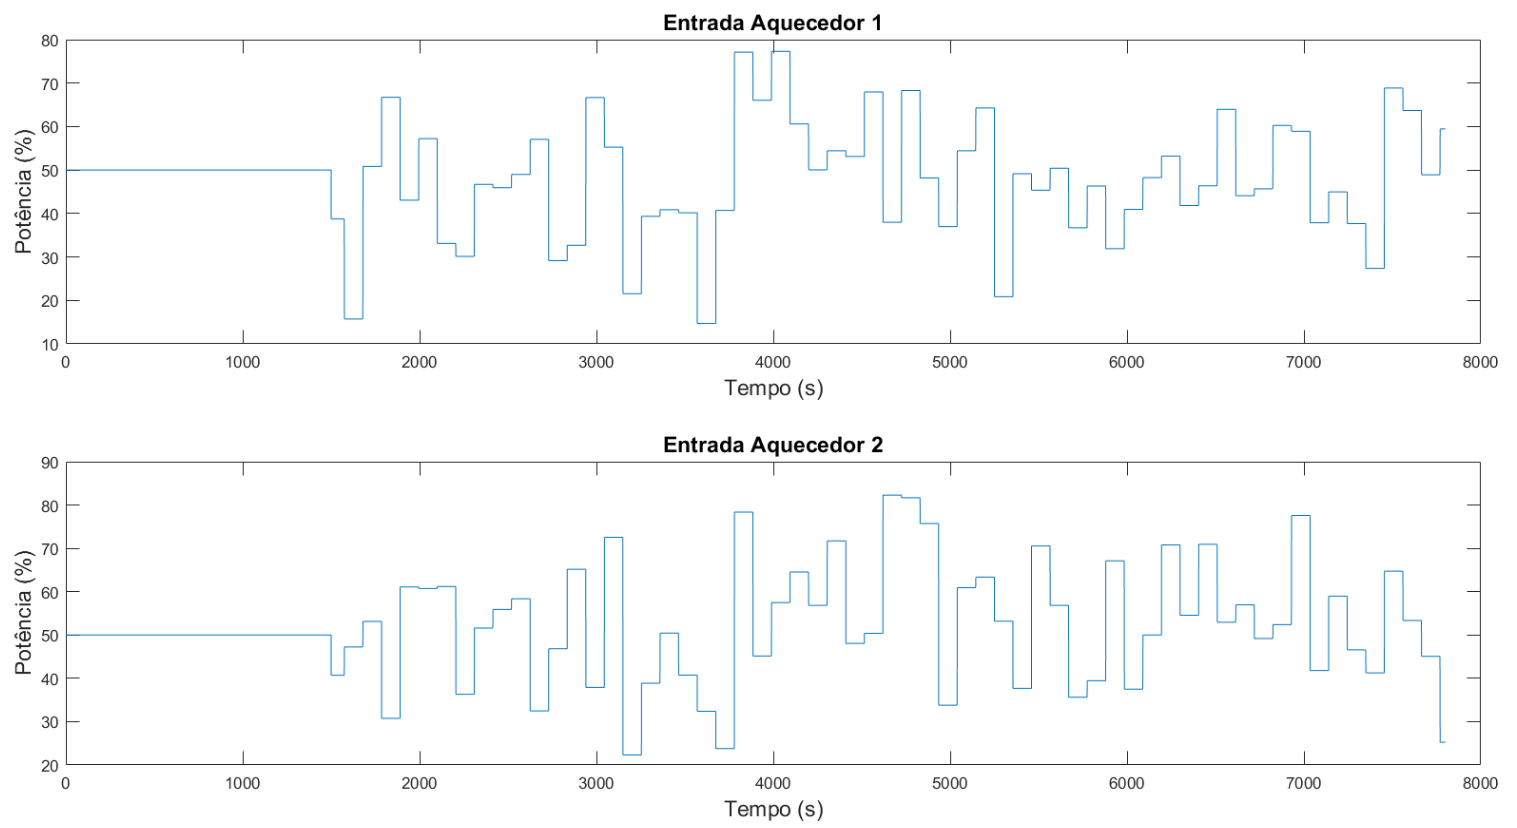
\includegraphics[width=0.95\textwidth]{./5_images/inputs_H1H2.png} 
		\label{fig:experiment_inputs}
	\end{center}
	\centering
	\makebox[\width]{Fonte: Autor} 
\end{figure}

% -----------------------------------------------------------------------------------------------------
% ------------------------------------------- Subsubsection -------------------------------------------
% -----------------------------------------------------------------------------------------------------
\subsubsection{Duração do experimento}
\label{subsubsec:duracao_do_experimento}

A duração do experimento, segundo \citeonline{Garcia2005}, deveria ser
a maior possível, uma vez que a variância das estimativas é proporcional ao inverso da duração do
experimento, porém sob o ponto de vista prático e experimental, a duração do experimento deveria ser
a menor possível para a obtenção de um modelo aceitável, pois ao longo do experimento o processo
estará sujeito a perturbações extras que podem impactar na operação da planta, na qualidade dos
produtos ou até na segurança do processo.

Cada um dos experimentos de coleta de dados do \acrshort{tclabsp} teve uma duração de $7800s$,
sendo que os $1500s$ iniciais foram utilizados para a estabilização do processo e os demais ($6300s$)
para as coletas. O critério utilizado para a determinação deste valor foi o de estimular a dinâmica
da planta aproximadamente $60x$ para cada um dos experimentos. Sabendo que os sinais de excitação
podem permanecer constantes por até $105s$ ($5T_s$), como mostrado na \cref{subsubsec:sinais_de_excitacao},
então temos a \cref{eq:experiment_duration}:

\begin{equation}
	\label{eq:experiment_duration}
	60 * 5T_s = \pmb{6}\pmb{3}\pmb{0}\pmb{0}\pmb{s}
\end{equation}

% .....................................................................................................
% ............................................ Subsection .............................................
% .....................................................................................................
\subsection{Definição do modelo experimental}
\label{subsec:definicao_modelo_experimental}

Esta seção apresenta mais algumas características teóricas importantes na definição de um modelo
que represente o sistema simulado e ao final dela, a \cref{subsubsec:modelo_experimental}
mostra a aplicação prática dessas características utilizando o conjunto de ferramentas do \acrshort{matlab}
para identificação de sistemas, o \textit{System Identification Toolbox\texttrademark}.

% -----------------------------------------------------------------------------------------------------
% ------------------------------------------- Subsubsection -------------------------------------------
% -----------------------------------------------------------------------------------------------------
\subsubsection{Escolha da representação matemática}
\label{subsubsec:escolha_da_representacao_matematica}

Existem diversas representações matemáticas distintas para modelos lineares, sendo que, segundo
\citeonline{Aguirre2015}, a mais utilizada é a função de transferência, porém \citeonline{Wang2009}
destaca que nos últimos anos tem se observado um aumento na popularidade dos modelos de espaço de
estados para desenvolvimento de controle preditivo. Para \citeonline{Aguirre2015} é importante ainda
salientar o modelo \acrshort{ar} (\acrlong{ar}), o modelo \acrshort{arx} (\acrlong{arx}) e
o modelo \acrshort{armax} (\acrlong{armax}).

\begin{citacao}
    \text{[...]} quando se trata da modelagem obtida por meios fenomenológicos é comum que se adote a base de
    tempo contínuo, em virtude de a maioria das leis da física serem expressas nesse tempo. Por sua vez,
    quando se trata de identificação de sistemas por processos experimentais, trabalha-se com amostras
    de dados coletados a cada intervalo de tempo, nesses casos usualmente adota-se o tempo discreto.
    \apud{Garcia2005}{Favaro2012}
\end{citacao}

% -----------------------------------------------------------------------------------------------------
% ------------------------------------------- Subsubsection -------------------------------------------
% -----------------------------------------------------------------------------------------------------
\subsubsection{Determinação da estrutura do modelos}
\label{subsubsec:determinacao_da_estrutura_do_modelo}

Determinar a ordem de um modelo é um dos aspectos mais importantes na determinação de sua estrutura,
uma vez que, caso sua ordem seja muito menor do que a ordem efetiva do sistema real, o modelo não
refletirá a completamente sua complexidade estrutural. Analogamente, escolher um modelo que a ordem
seja muito maior do que a necessária, provavelmente causará uma estimação de parâmetros mal condicionada.
\cite{Aguirre2015}

Neste trabalho será utilizado o \textit{critério de informação de Akaike} \apud{Akaike1974}{Aguirre2015}
(\acrshort{aic}), definido por:

\begin{equation}
	\label{eq:aic}
	AIC(n_\theta) = N \ln \left[ \sigma_{erro}^2 (n_\theta) \right] + 2n_\theta
\end{equation}

\noindent
Onde: 
\begin{itemize}
	\item $N$: é o número de dados
	\item $\sigma_{erro}^2 (n_\theta)$: é a variância dos resíduos
	\item $n_\theta = \mathrm{dim}[\hat{\theta}]$: é o número de parâmetros do modelo
\end{itemize}

Segundo \citeonline{Aguirre2015} a utilização deste critério na escolha da estrutura do modelo se justifica
pois à medida que termos são incluídos no modelo, o número de graus de liberdade aumenta, permitindo
um ajuste de dados mais exato. Resumidamente, a primeira parcela da equação quantifica a diminuição
da variância dos resíduos resultante da inclusão de um termo, ao passo que a segunda parcela penaliza
a inclusão de cada termo.

O índice \acrshort{aic}($n_\theta$) normalmente atinge um mínimo para um determinado número de parâmetros
no modelo $n_{\theta}^*$, e, ainda segundo \citeonline{Aguirre2015}, do ponto de vista do critério utilizado,
esse número de parâmetros é ótimo.

% -----------------------------------------------------------------------------------------------------
% ------------------------------------------- Subsubsection -------------------------------------------
% -----------------------------------------------------------------------------------------------------
\subsubsection{Estimação de parâmetros}
\label{subsubsec:estimacao_de_parametros}

A estimação de parâmetros, segundo \apudonline{Eykhoff1974}{Favaro2012} é a determinação experimental
de valores de parâmetros que governam a dinâmica e/ou o comportamento não-linear, assumindo que a
estrutura do modelo seja conhecida.

Essa etapa começa com a escolha do algoritmo a ser utilizado \cite{Aguirre2015}. Dentre eles, os
mais amplamente empregados na literatura são: método da análise de frequência; método da resposta
transitória e método dos mínimos quadrados \cite{Favaro2012}.

Como será visto na \cref{subsubsec:modelo_experimental}, neste trabalho diversas representações matemáticas
distintas foram testadas, e para cada uma delas foi utilizada uma função do \acrshort{matlab} para 
a estimação automática de parâmetros. A \cref{tab:param_est_functions} identifica as funções
utilizadas em cada uma das representações distintas\footnote{
    Documentações das funções disponíveis em:

    $\mathtt{tfest}$ - \url{https://www.mathworks.com/help/ident/ref/tfest.html}

    $\mathtt{ssest}$ - \url{https://www.mathworks.com/help/ident/ref/ssest.html}

    $\mathtt{arx}$ - \url{https://www.mathworks.com/help/ident/ref/arx.html}

    $\mathtt{armax}$ - \url{https://www.mathworks.com/help/ident/ref/armax.html}

    $\mathtt{oe}$ - \url{https://www.mathworks.com/help/ident/ref/oe.html}

    $\mathtt{bj}$ - \url{https://www.mathworks.com/help/ident/ref/bj.html}

    $\mathtt{nlarx}$ - \url{https://www.mathworks.com/help/ident/ref/nlarx.html}
}.

\begin{table}[h]
	\centering
	\caption{Funções para a estimação de parâmetros}
	\label{tab:param_est_functions}
	\begin{tabular}{ll} \toprule
		{Representação matemática}		                                & {Função}				                    \\ \midrule
		Função de transferência		                                    & $\mathtt{tfest}$                          \\
		Espaço de estados   		                                    & $\mathtt{ssest}$                          \\
		\acrshort{arx}		                                            & $\mathtt{arx}$                            \\
		\acrshort{armax}		                                        & $\mathtt{armax}$                          \\
		Erro de saída (\acrshort{oe}, do inglês \acrlong{oe})		    & $\mathtt{oe}$                             \\
		\acrlong{bj} (\acrshort{bj})             	                    & $\mathtt{bj}$                             \\
		\acrshort{arx} não-linear (\acrshort{nlarx})                    & $\mathtt{nlarx}$                          \\ \bottomrule
	\end{tabular}
	\caption*{Fonte: Autor}
\end{table}

% -----------------------------------------------------------------------------------------------------
% ------------------------------------------- Subsubsection -------------------------------------------
% -----------------------------------------------------------------------------------------------------
\subsubsection{Validação do modelo}
\label{subsubsec:validacao_do_modelo}

Em problemas de validação, a questão é tentar determinar se um dado modelo é válido ou não e para isso,
deve-se simulá-lo sem qualquer ajuste adicional e compará-lo a dados medidos em testes diferentes daquele
usado no desenvolvimento da sintonia do mesmo. A motivação para tal cuidado deve-se ao fato de desejar-se
saber o quão geral é o modelo. Portanto, esta divisão entre os dados de treinamento e de validação refere-se
à \textit{capacidade de generalização do modelo} \cite{Aguirre2015}.

A proporção entre dados de treinamento e validação utilizada neste trabalho é de 60\% para dados de treinamento
e 40\% para validação. Para realizar a comparação entre o modelo obtido e os dados de validação, utilizou-se
a função \texttt{compare} no \acrshort{matlab}.

Esta função \texttt{compare} avalia o quanto o modelo obtido se encaixa aos dados de validação calculando
o erro do quadrado médio da raiz normalizada, assim como descrito na \cref{eq:nrmse} a seguir:

\begin{equation}
	\label{eq:nrmse}
	\mathrm{fit} = 100 \left( 1 - \frac{ \| y - \hat{y} \| }{ \| y - \mathrm{média}(y) \| } \right)
\end{equation}

\noindent
Onde: 
\begin{itemize}
	\item $y$: são os dados de validação
	\item $\hat{y}$: são os dados do modelo
\end{itemize}

Também neste trabalho aplica-se o teste de \textit{análise de resíduos} dos modelos estudados e a motivação
para tal pode ser melhor compreendida nas palavras de \citeonline{Aguirre2015} a seguir:

\begin{citacao}
    \text{[...]} Do ponto de vista da validação de modelos, a motivação de se verificar quão são aleatórios
    os resíduos pode ser entendida lembrando que os resíduos são a parte dos dados que o modelo não
    consegue explicar. Exigir que o modelo explique os dados em todos os seus detalhes é, no mínimo,
    ingênuo. Mas quanto dos dados precisa ser explicado? O modelo deve explicar \textit{tudo que for
    explicável nos dados}. Se isso ocorrer, então os resíduos conterão apenas aquilo que não é explicável e,
    portanto, serão brancos. Assim, se os resíduos forem brancos, não há informação útil neles, ou seja,
    o modelo explicou tudo que era possível explicar. \text{[...]} 
\end{citacao}

Para tal teste utiliza-se a função \texttt{resid} no \acrshort{matlab}.

% -----------------------------------------------------------------------------------------------------
% ------------------------------------------- Subsubsection -------------------------------------------
% -----------------------------------------------------------------------------------------------------
\subsubsection{Modelos experimentais}
\label{subsubsec:modelo_experimental}

Esta seção apresenta maiores detalhes práticos dos procedimentos descritos nas 
\crefrange{subsubsec:escolha_da_representacao_matematica}{subsubsec:validacao_do_modelo} e os
\textit{scripts} de \acrshort{matlab} utilizados para a obtenção dos resultados também serão
apresentados e discutidos ao longo do texto.

Após as coletas de dados descritas das
\crefrange{subsec:testes_dinamicos_e_coleta_de_dados}{subsubsec:duracao_do_experimento}
preparou-se então no \acrshort{matlab} um objeto do tipo \texttt{iddata} contendo os dados dos aquecedores
e dos sensores de temperatura do \acrshort{tclabsp}.
Esses dados foram divididos em 2 grupos: identificação e validação, como já visto na \cref{subsubsec:validacao_do_modelo}.
As entradas e saídas do sistema, subdivididas nesses 2 grupos, foram criadas a partir do código-fonte
\ref{lst:tclabsp-model-iddata} e podem ser observadas na \cref{fig:tclabsp-model-IOs}.

\begin{figure}[h]
	\caption{Entradas e saídas coletadas em ensaios no \acrshort{tclabsp}}
	\begin{center}
		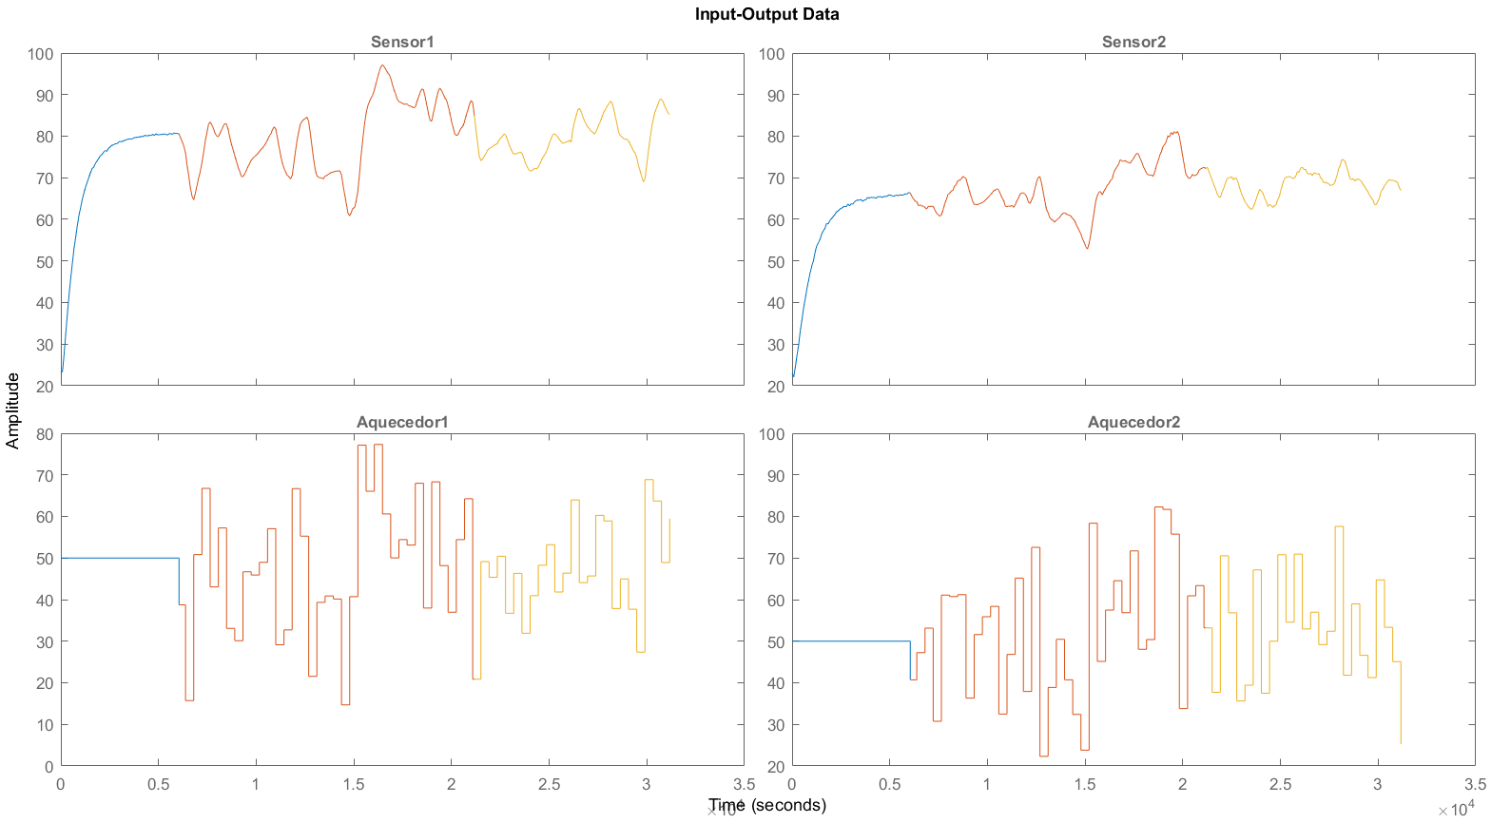
\includegraphics[width=1.00\textwidth]{./5_images/tclabsp-model-IOs.png} 
		\label{fig:tclabsp-model-IOs}
	\end{center}
	\centering
	\makebox[\width]{Fonte: Autor} 
\end{figure}

Na \cref{fig:tclabsp-model-IOs} é possível observar 3 conjuntos de dados distintos, indicados pelas cores 
azul, vermelho e laranja. Os dados em \textbf{azul} foram descartados, pois representam o período de 
estabilização do sistema em 50\% dos aquecedores. Os dados em \textbf{vermelho} e \textbf{laranja} representam
os dados de identificação e validação, respectivamente.

\lstinputlisting[	
	caption={Criação dos conjuntos de identificação e validação para o sistema \acrshort{tclabsp}},
	captionpos=t,
    label={lst:tclabsp-model-iddata},
    firstline=1,
    lastline=55,
    language=Matlab,
	style=Matlab_lang]
	{D:/Repos/TCLabSP/Simulink (MATLAB R2016a)/02-ModeloExperimental/RunMe.m}
	\begin{center}
		\makebox[\width]{Fonte: Autor}
    \end{center}
% TODO: Substituir endereço do arquivo

Com o intuito fazer diversos testes e de avaliar muitos modelos diferentes, utilizou-se um
\textit{script} para a criação automática de modelos experimentais baseados nos dados mostrados
na \cref{fig:tclabsp-model-IOs}. Este \textit{script} utiliza as funções descritas na \cref{tab:param_est_functions}
e seu código-fonte pode ser visto no \cref{sec:tclabsp-models-creation}. 
A \cref{tab:tclabsp-models-description} apresenta a quantidade de modelos que foram gerados a partir dele.

\begin{table}[h]
	\centering
	\caption{Modelos experimentais do \acrshort{tclabsp}}
	\label{tab:tclabsp-models-description}
	\begin{tabular}{ll} \toprule
		{Representação matemática}		                                & {Quantidade}          \\ \midrule
		Função de transferência		                                    & $10.000$              \\
		Espaço de estados   		                                    & $10$                  \\
		\acrshort{arx}		                                            & $80$                  \\
		\acrshort{armax}		                                        & $320$                 \\
		\acrshort{oe}													& $80$                  \\
		\acrshort{bj}                                   				& $1.280$               \\
		\acrshort{nlarx}                    							& $26.244$              \\ \bottomrule
	\end{tabular}
	\caption*{Fonte: Autor}
\end{table}

% _____________________________________________________________________________________________________
% ___________________________________________ Paragraph _______________________________________________
% _____________________________________________________________________________________________________
\paragraph*{\textbf{Modelos experimentais de função de transferência}}
\label{par:modelos_experimentais_tf}

Os modelos experimentais criados na forma de função de transferência foram obtidos a partir de diversas combinações
entre a quantidade de pólos e zeros nos subsistemas existentes entre os Sensores 1 e 2, e entre os Aquecedores 1 e 2.
Essas combinações são descridas na \cref{tab:tclabsp-models-tf}.

\begin{table}[h]
	\centering
	\caption{Modelos experimentais - Função de transferência}
	\label{tab:tclabsp-models-tf}
	\begin{tabular}{l|l|l|}
        \cline{2-3}
                                                & \textbf{Aquecedor 1}                                                      & \textbf{Aquecedor 2}                                                      \\ \hline
        \multicolumn{1}{|l|}{\textbf{Sensor 1}} & \begin{tabular}[c]{@{}l@{}}pólos: de 2 a 5\\ zeros: de 1 a 4\end{tabular} & \begin{tabular}[c]{@{}l@{}}pólos: de 2 a 5\\ zeros: de 1 a 4\end{tabular} \\ \hline
        \multicolumn{1}{|l|}{\textbf{Sensor 2}} & \begin{tabular}[c]{@{}l@{}}pólos: de 2 a 5\\ zeros: de 1 a 4\end{tabular} & \begin{tabular}[c]{@{}l@{}}pólos: de 2 a 5\\ zeros: de 1 a 4\end{tabular} \\ \hline
    \end{tabular}
	\caption*{Fonte: Autor}
\end{table}

Para cada uma das combinações possíveis descritas na \cref{tab:tclabsp-models-tf} foi criado um modelo utilizando o
conjunto de dados de identificação. Esses modelos foram testados com o conjunto de dados de validação através da \cref{eq:nrmse}
e o resultado destes testes, juntamente com o critério de \acrshort{aic}, podem ser observados na \cref{fig:tclabsp-models-tf}.

\begin{figure}[h]
	\caption{Modelos experimentais de função de transferência}
	\begin{center}
		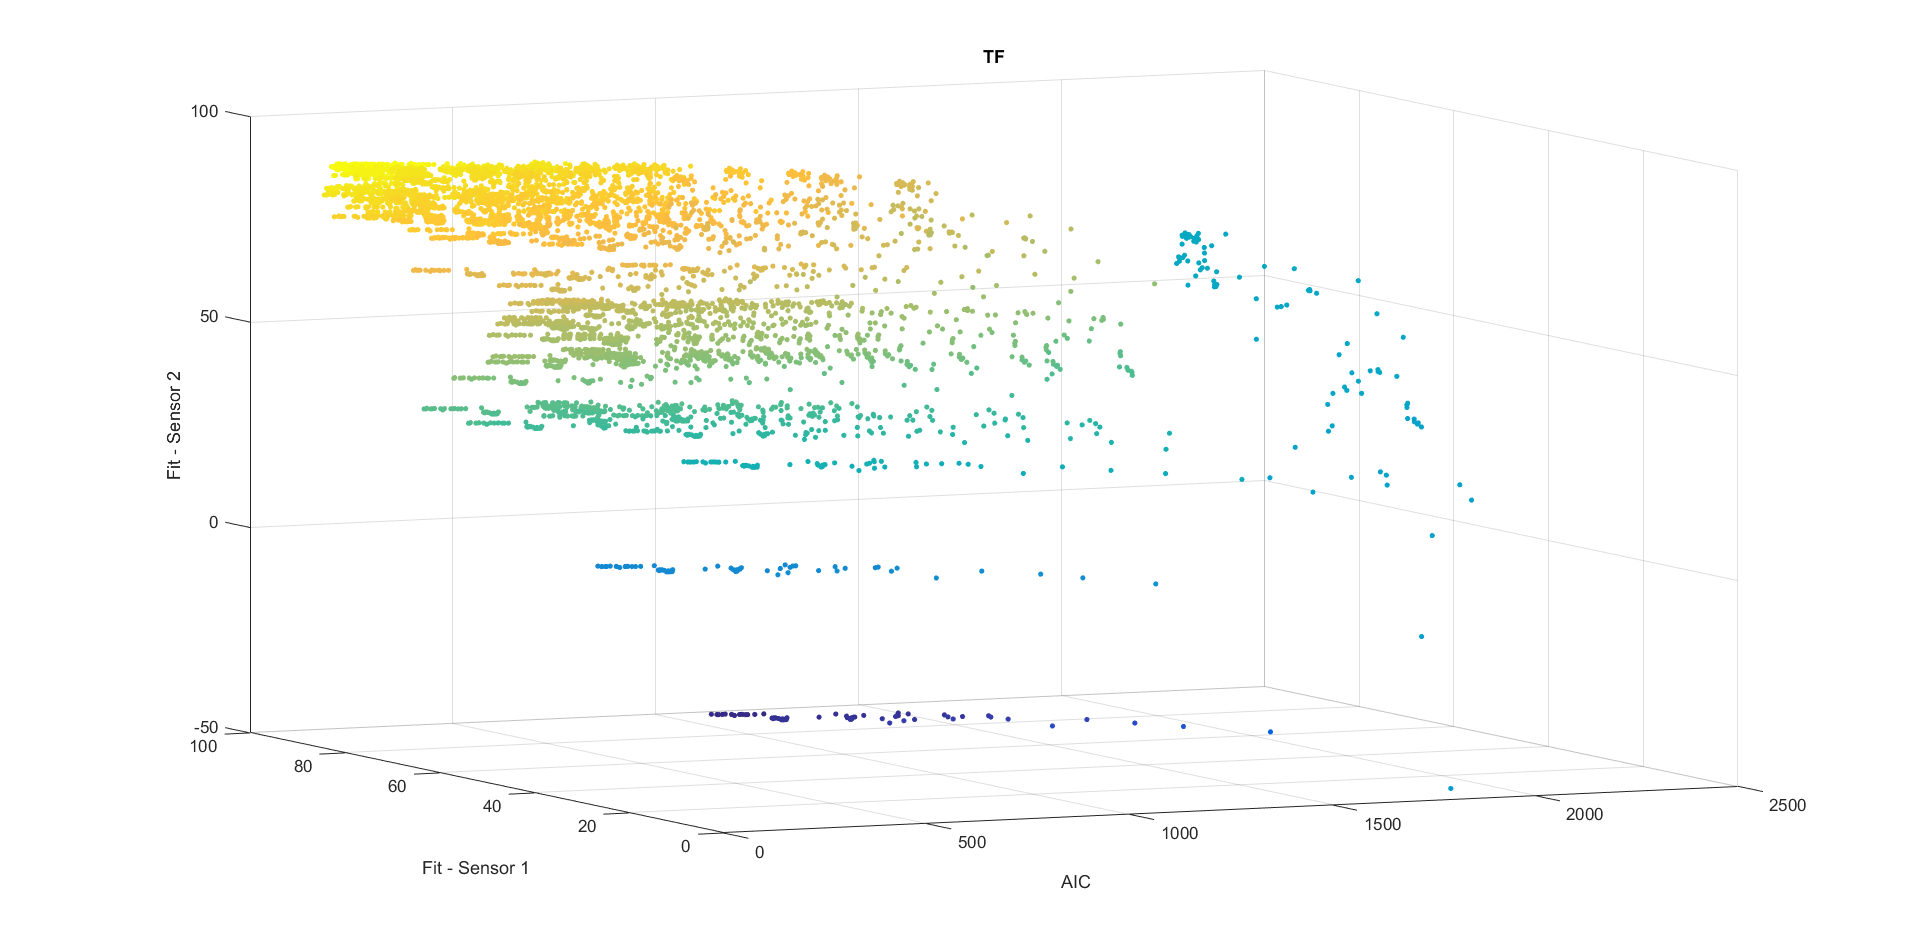
\includegraphics[width=1.00\textwidth]{./5_images/tclabsp-models-TF.png} 
		\label{fig:tclabsp-models-tf}
	\end{center}
	\centering
	\makebox[\width]{Fonte: Autor} 
\end{figure}

Cada um dos pontos presentes na \cref{fig:tclabsp-models-tf} representam um modelo experimental diferente, sendo que as cores
mais claras indicam aqueles com menor erro quando comparados ao conjunto de dados de validação.

A fim de escolher o melhor modelo de função de transferência frente aos 10000 gerados, os 10 primeiros modelos com menor 
valor segundo o critério de \acrshort{aic} foram submetidos à análise de resíduos (vide \cref{subsubsec:validacao_do_modelo}) e
dentre eles o que mostrou menor valor na análise resídual foi o modelo descrito na \cref{tab:tclabsp-model-tf}.
O teste deste modelo junto aos dados de validação e sua análise de resíduos podem ser visualizadas nas
\cref{fig:tclabsp-models-tf-compare,fig:tclabsp-models-tf-resid}, respectivamente.

\begin{table}[h]
	\centering
	\caption{Melhor modelo experimental - Função de transferência}
	\label{tab:tclabsp-model-tf}
	\begin{tabular}{c|c} \toprule
		{Entradas e saídas}		                                            & {Função de transferência}                                                                                                                                 \\ \midrule
        \begin{tabular}[c]{@{}l@{}}Aquecedor 1\\Sensor 1\end{tabular}		& $\frac{ 0.1248 z^{-1} - 0.01046 z^{-2} - 0.1142 z^{-3} }{ 1 - 0.8092 z^{-1} - 1.03 z^{-2} + 0.7405 z^{-3} + 0.1342 z^{-4} - 0.03503 z^{-5} }$             \\ \midrule
		\begin{tabular}[c]{@{}l@{}}Aquecedor 1\\Sensor 2\end{tabular}  		& $\frac{ 0.007869 z^{-1} - 0.007693 z^{-2} }{ 1 - 1.985 z^{-1} + 0.2452 z^{-2} + 1.659 z^{-3} - 1.083 z^{-4} + 0.1637 z^{-5} }$                            \\ \midrule
		\begin{tabular}[c]{@{}l@{}}Aquecedor 2\\Sensor 1\end{tabular}		& $\frac{ 0.00452 z^{-1}+ 0.005953 z^{-2} }{ 1 - 0.2164 z^{-1} - 1.301 z^{-2} + 0.2197 z^{-3} + 0.4412 z^{-4} - 0.08218 z^{-5} }$                           \\ \midrule
		\begin{tabular}[c]{@{}l@{}}Aquecedor 2\\Sensor 2\end{tabular}       & $\frac{ 0.06374 z^{-1} - 0.04266 z^{-2} }{ 1 - 1.504 z^{-1} + 0.4851 z^{-2} + 0.2172 z^{-3} - 0.2665 z^{-4} + 0.12 z^{-5} }$                              \\ \bottomrule
	\end{tabular}
	\caption*{Fonte: Autor}
\end{table}

\begin{figure}[h]
	\caption{Modelo: função de transferência - Teste de validação}
	\begin{center}
		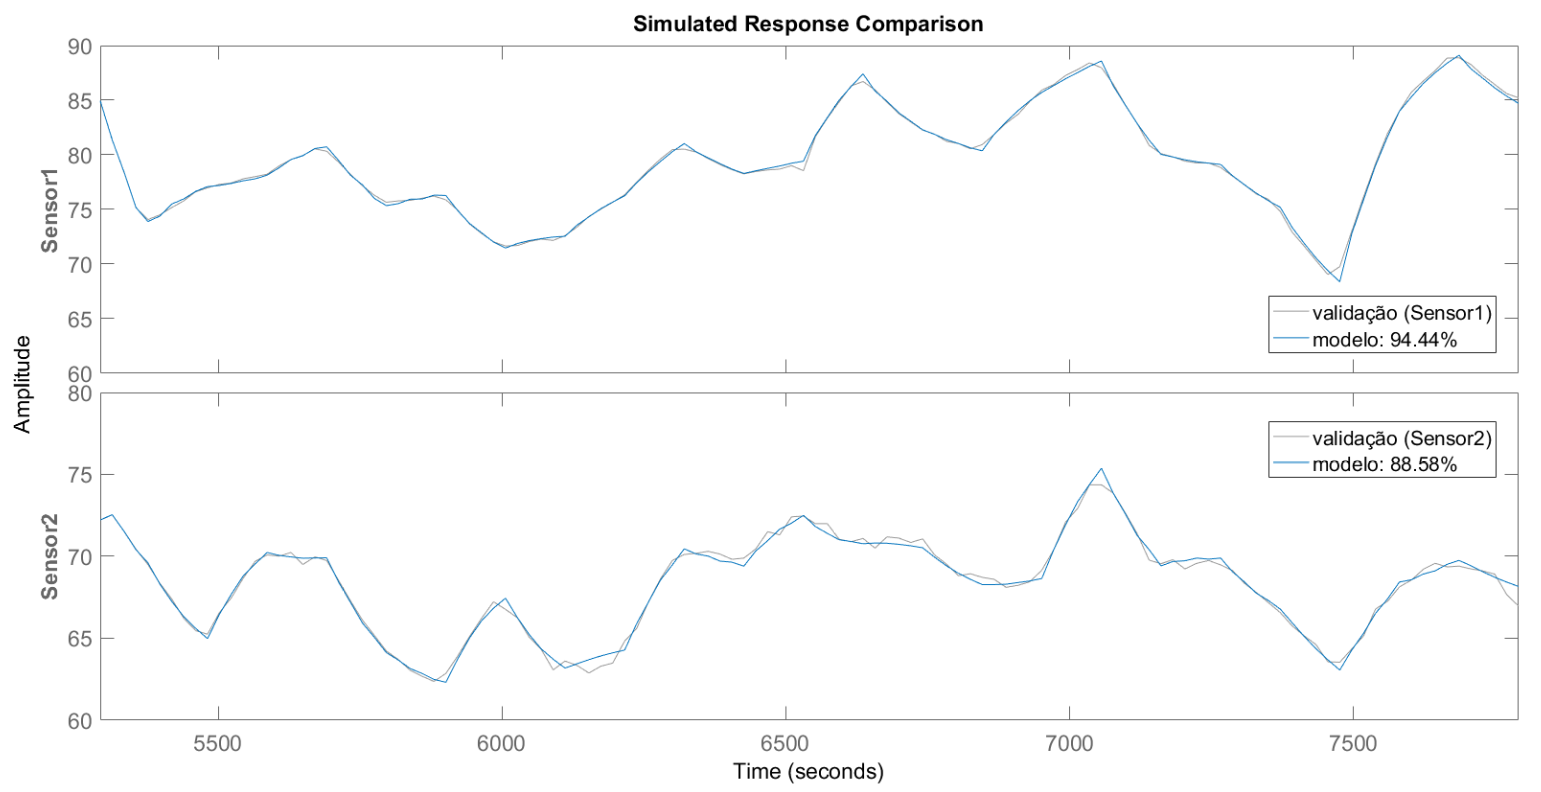
\includegraphics[width=1.00\textwidth]{./5_images/tclabsp-models-TF-compare.png} 
		\label{fig:tclabsp-models-tf-compare}
	\end{center}
	\centering
	\makebox[\width]{Fonte: Autor} 
\end{figure}

\begin{figure}[h]
	\caption{Modelo: função de transferência - Análise de resíduos}
	\begin{center}
		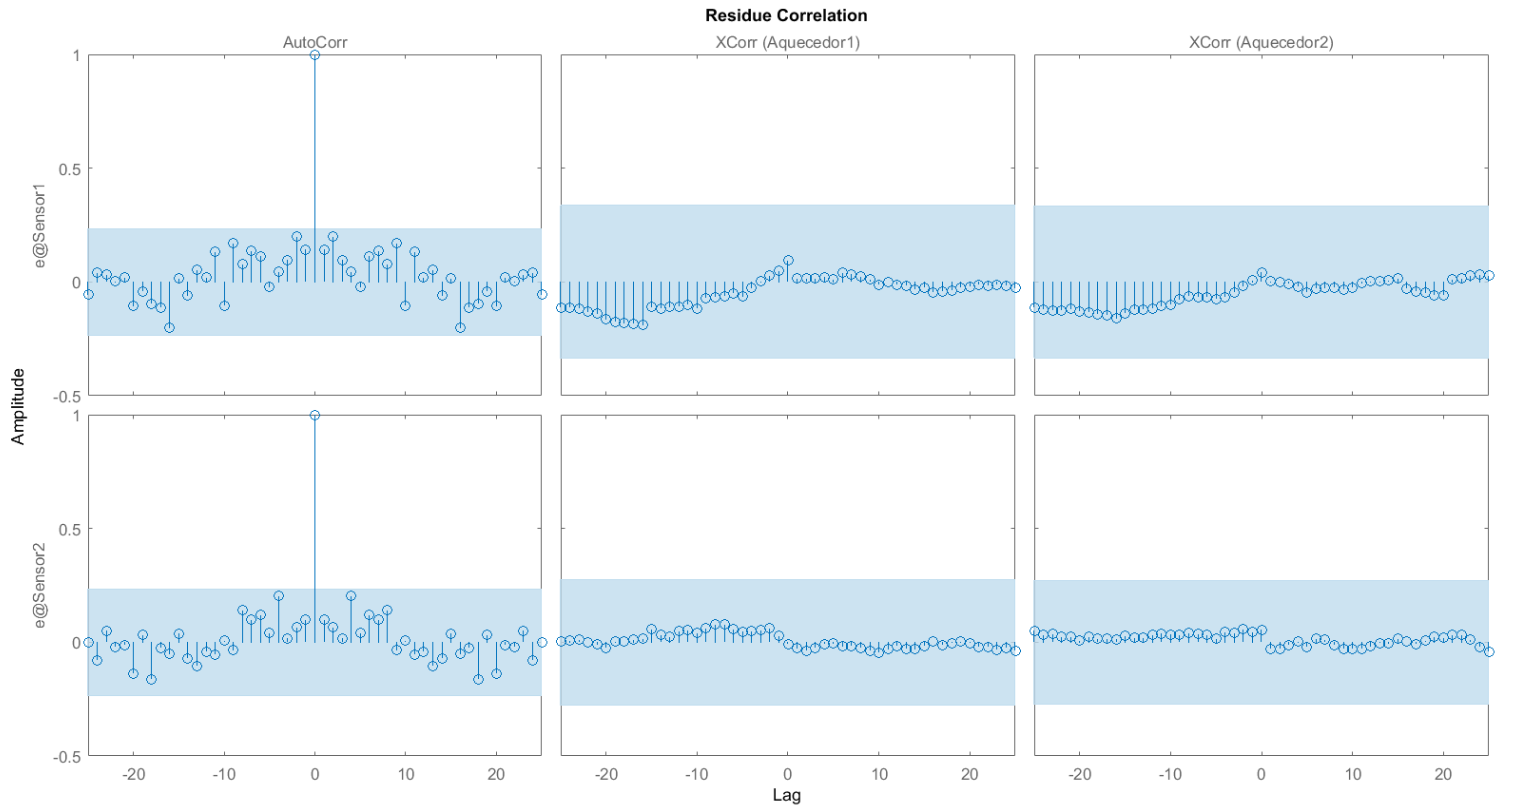
\includegraphics[width=1.00\textwidth]{./5_images/tclabsp-models-TF-resid.png} 
		\label{fig:tclabsp-models-tf-resid}
	\end{center}
	\centering
	\makebox[\width]{Fonte: Autor} 
\end{figure}

% _____________________________________________________________________________________________________
% ___________________________________________ Paragraph _______________________________________________
% _____________________________________________________________________________________________________
\paragraph*{\textbf{Modelos experimentais de espaço de estados}}
\label{par:modelos_experimentais_ss}

Para a escolha do modelo experimental em espaço de estados foram testados 10 modelos de ordens distintas,
entre as ordens 1 e 10, e gráfico mostrando a comparação destes modelos frente ao critério de \acrshort{aic}
e aos dados de validação dos sensores 1 e 2 pode ser observado na \cref{fig:tclabsp-models-ss}.

\begin{figure}[h]
	\caption{Modelos experimentais de espeço de estados}
	\begin{center}
		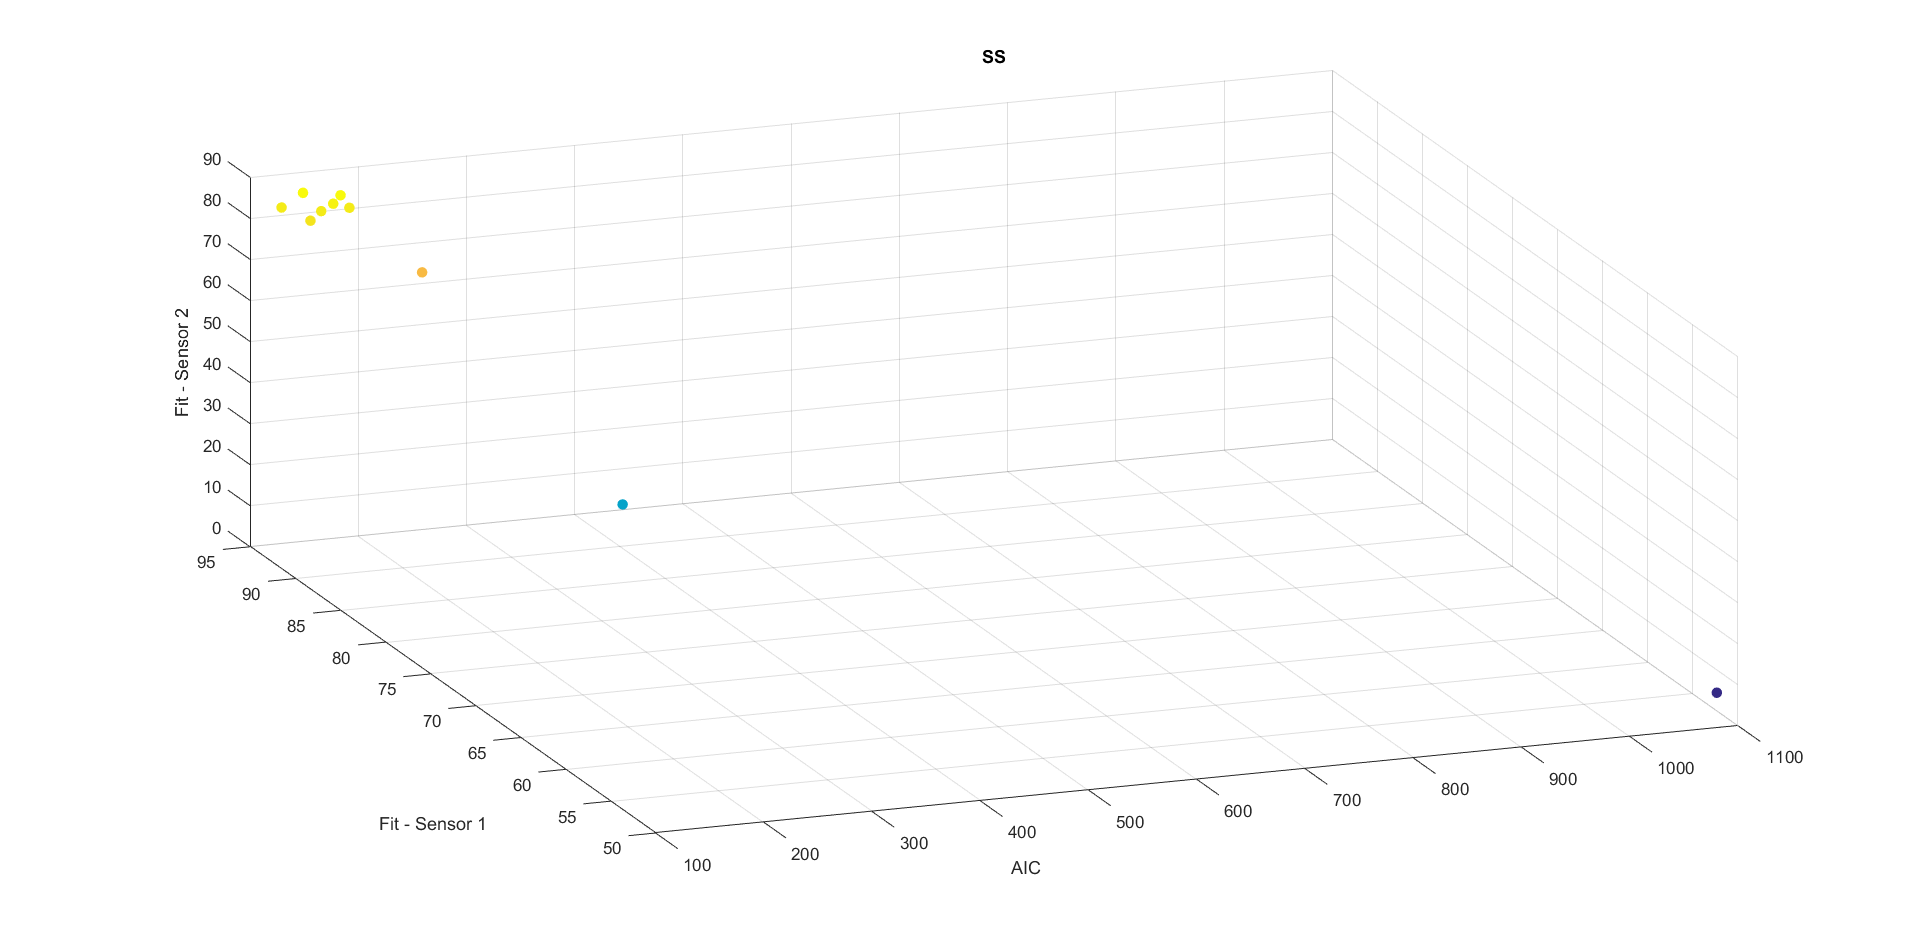
\includegraphics[width=1.00\textwidth]{./5_images/tclabsp-models-SS.png} 
		\label{fig:tclabsp-models-ss}
	\end{center}
	\centering
	\makebox[\width]{Fonte: Autor} 
\end{figure}

Dentre todos os testados, o modelo de ordem 3 apresentou o menor valor no critério de \acrshort{aic} e foi
selecionado. O formato e as matrizes deste modelo podem ser vistos na \cref{eq:tclabsp-model-ss}
e o gráfico de teste junto aos dados de validação na \cref{fig:tclabsp-models-ss-compare}.

\begin{equation}
	\label{eq:tclabsp-model-ss}
	\begin{aligned}
		x(t + T_s) &= Ax(t) + Bu(t) + Ke(t)	\\
		y(t) &= Cx(t) + Du(t) + e(t)		\\
	\end{aligned}
\end{equation}

\begin{equation*}
	\begin{aligned}
		A &= \bbordermatrix{
											&	\textcolor{matrixtitle}{x_1}	&	\textcolor{matrixtitle}{x_2}	&	\textcolor{matrixtitle}{x_3}	\cr
			\textcolor{matrixtitle}{x_1}	&	0.9099							&	-0.02543						&	-0.02673	 					\cr
			\textcolor{matrixtitle}{x_2}	&	-0.06169						&	0.8193							&	-0.01098	 					\cr
			\textcolor{matrixtitle}{x_3}	&	-0.03506						&	0.108							&	0.9884		 					\cr
		}
		, \\
		C &= \bbordermatrix{
												&	\textcolor{matrixtitle}{x_1}	&	\textcolor{matrixtitle}{x_2}	&	\textcolor{matrixtitle}{x_3}	\cr
			\textcolor{matrixtitle}{Sensor_1}	&	180.1							&	8.69							&	1.814							\cr
			\textcolor{matrixtitle}{Sensor_2}	&	159.2							&	-40.71							&	1.665							\cr
		}
		,
	\end{aligned}
	\begin{aligned}
		B &= \bbordermatrix{
											&	\textcolor{matrixtitle}{Aquecedor_1}	&	\textcolor{matrixtitle}{Aquecedor_2}	\cr
			\textcolor{matrixtitle}{x_1}	&	0.0005512								&	7.033 \times 10^{-5}					\cr
			\textcolor{matrixtitle}{x_2}	&	0.002047								&	-0.001209								\cr
			\textcolor{matrixtitle}{x_3}	&	-0.0009257								&	0.0009081								\cr
		}
		, \\
		D &= \bbordermatrix{
												&	\textcolor{matrixtitle}{Aquecedor_1}	&	\textcolor{matrixtitle}{Aquecedor_2}	\cr
			\textcolor{matrixtitle}{Sensor_1}	&	0           							&	0										\cr
			\textcolor{matrixtitle}{Sensor_2}	&	0           							&	0										\cr
		}
		,
	\end{aligned}
\end{equation*}

\begin{equation*}
	K = \bbordermatrix{
										&	\textcolor{matrixtitle}{Sensor_1}	&	\textcolor{matrixtitle}{Sensor_2}	\cr
		\textcolor{matrixtitle}{x_1}	&	0.000946							&	0.0008267							\cr
		\textcolor{matrixtitle}{x_2}	&	0.0006276							&	0.001956							\cr
		\textcolor{matrixtitle}{x_3}	&	-0.008009							&	0.003641							\cr
	}
\end{equation*}

\begin{figure}[h]
	\caption{Modelo: espaço de estados - Teste de validação}
	\begin{center}
		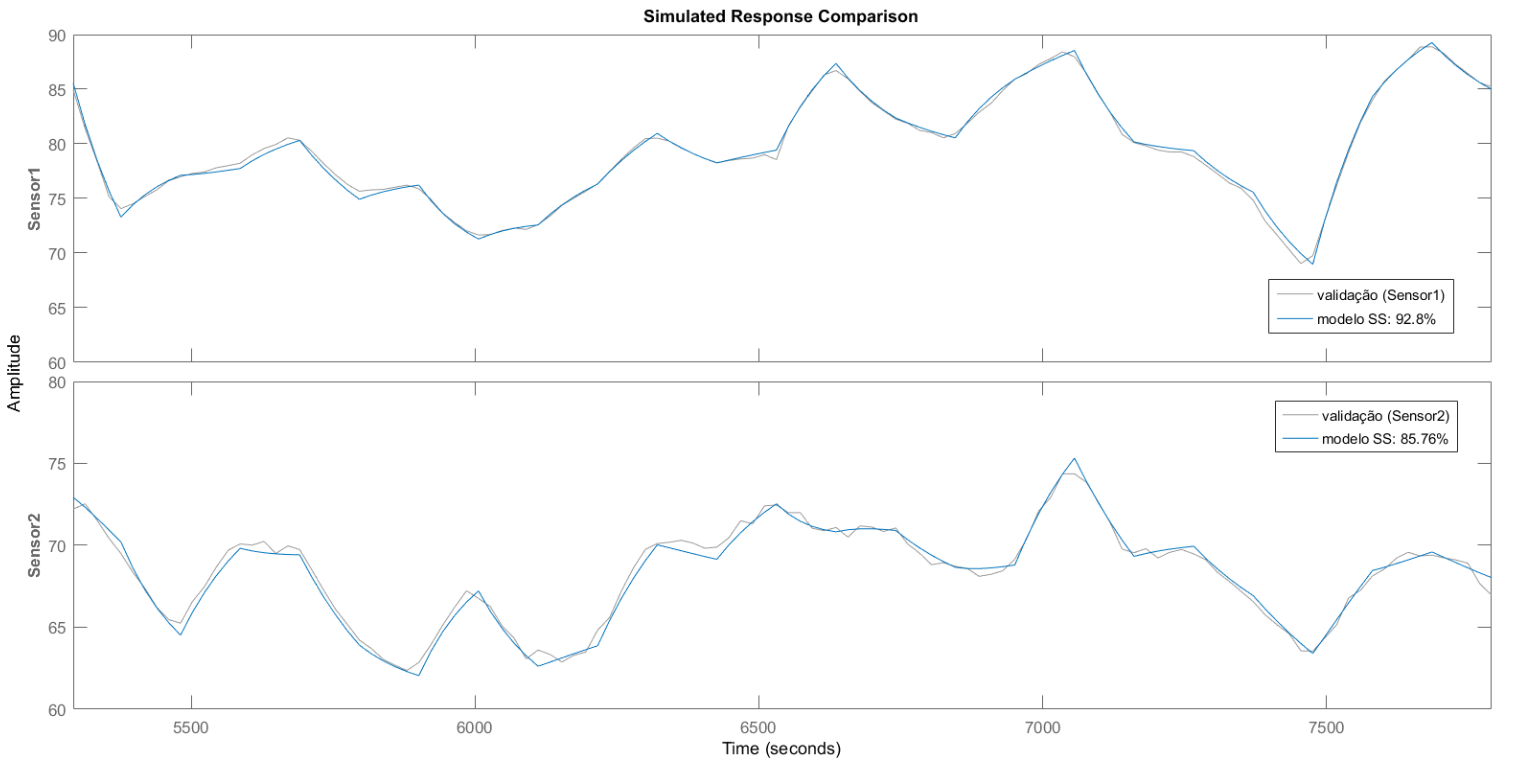
\includegraphics[width=1.00\textwidth]{./5_images/tclabsp-models-SS-compare.png} 
		\label{fig:tclabsp-models-ss-compare}
	\end{center}
	\centering
	\makebox[\width]{Fonte: Autor} 
\end{figure}

% _____________________________________________________________________________________________________
% ___________________________________________ Paragraph _______________________________________________
% _____________________________________________________________________________________________________
\paragraph*{\textbf{Modelos experimentais ARX}}
\label{par:modelos_experimentais_arx}

Os modelos \acrshort{arx} foram criados a partir de combinações de diferentes números de pólos ($n_a$),
números de zeros ($n_b$) e de tempo morto ($n_k$). As combinações utilizadas podem ser vistas na
\cref{tab:tclabsp-models-arx}.

\begin{table}[h]
	\centering
	\caption{Modelos experimentais - ARX}
	\label{tab:tclabsp-models-arx}
	\begin{tabular}{c|c} \toprule
		{Parâmetro}		&	{Valores utilizados nas combinações}									\\ \midrule
		$n_a$			&
							$ \begin{bmatrix}	1	&	1	\\	1	&	1	\\	\end{bmatrix} $	,		
							$ \begin{bmatrix}	2	&	2	\\	2	&	2	\\	\end{bmatrix} $	,		
							$ \begin{bmatrix}	3	&	3	\\	3	&	3	\\	\end{bmatrix} $	,		
							$ \begin{bmatrix}	4	&	4	\\	4	&	4	\\	\end{bmatrix} $		\\ \midrule
		$n_b$			&
							$ \begin{bmatrix}	1	&	1	\\	1	&	1	\\	\end{bmatrix} $	,		
							$ \begin{bmatrix}	2	&	2	\\	2	&	2	\\	\end{bmatrix} $	,		
							$ \begin{bmatrix}	3	&	3	\\	3	&	3	\\	\end{bmatrix} $	,		
							$ \begin{bmatrix}	4	&	4	\\	4	&	4	\\	\end{bmatrix} $		\\ \midrule
		$n_k$			&
							$ \begin{bmatrix}	0	&	0	\\	0	&	0	\\	\end{bmatrix} $	,		
							$ \begin{bmatrix}	1	&	1	\\	1	&	1	\\	\end{bmatrix} $	,		
							$ \begin{bmatrix}	2	&	2	\\	2	&	2	\\	\end{bmatrix} $	,		
							$ \begin{bmatrix}	3	&	3	\\	3	&	3	\\	\end{bmatrix} $	,		
							$ \begin{bmatrix}	4	&	4	\\	4	&	4	\\	\end{bmatrix} $		\\ \bottomrule
	\end{tabular}
	\caption*{Fonte: Autor}
\end{table}

A partir de todos os modelos possíveis gerados a partir das combinações dos parâmetros da \cref{tab:tclabsp-models-arx},
selecionou-se então os 10 modelos com menor valor segundo o critério de \acrshort{aic} e deste foi então
selecionado o modelo com menor valor residual.
O gráfico mostrando a distribuição dos modelos gerados em comparação ao critério de \acrshort{aic} pode ser
visto na \cref{fig:tclabsp-models-arx} e o modelo \acrshort{arx} escolhido, seu gráfico comparativo aos dados validação
e sua análise residual podem ser vistos na \cref{tab:tclabsp-model-arx}, na \cref{fig:tclabsp-models-arx-compare} e na
\cref{fig:tclabsp-models-arx-resid}, respectivamente.

\begin{figure}[h]
	\caption{Modelos experimentais ARX}
	\begin{center}
		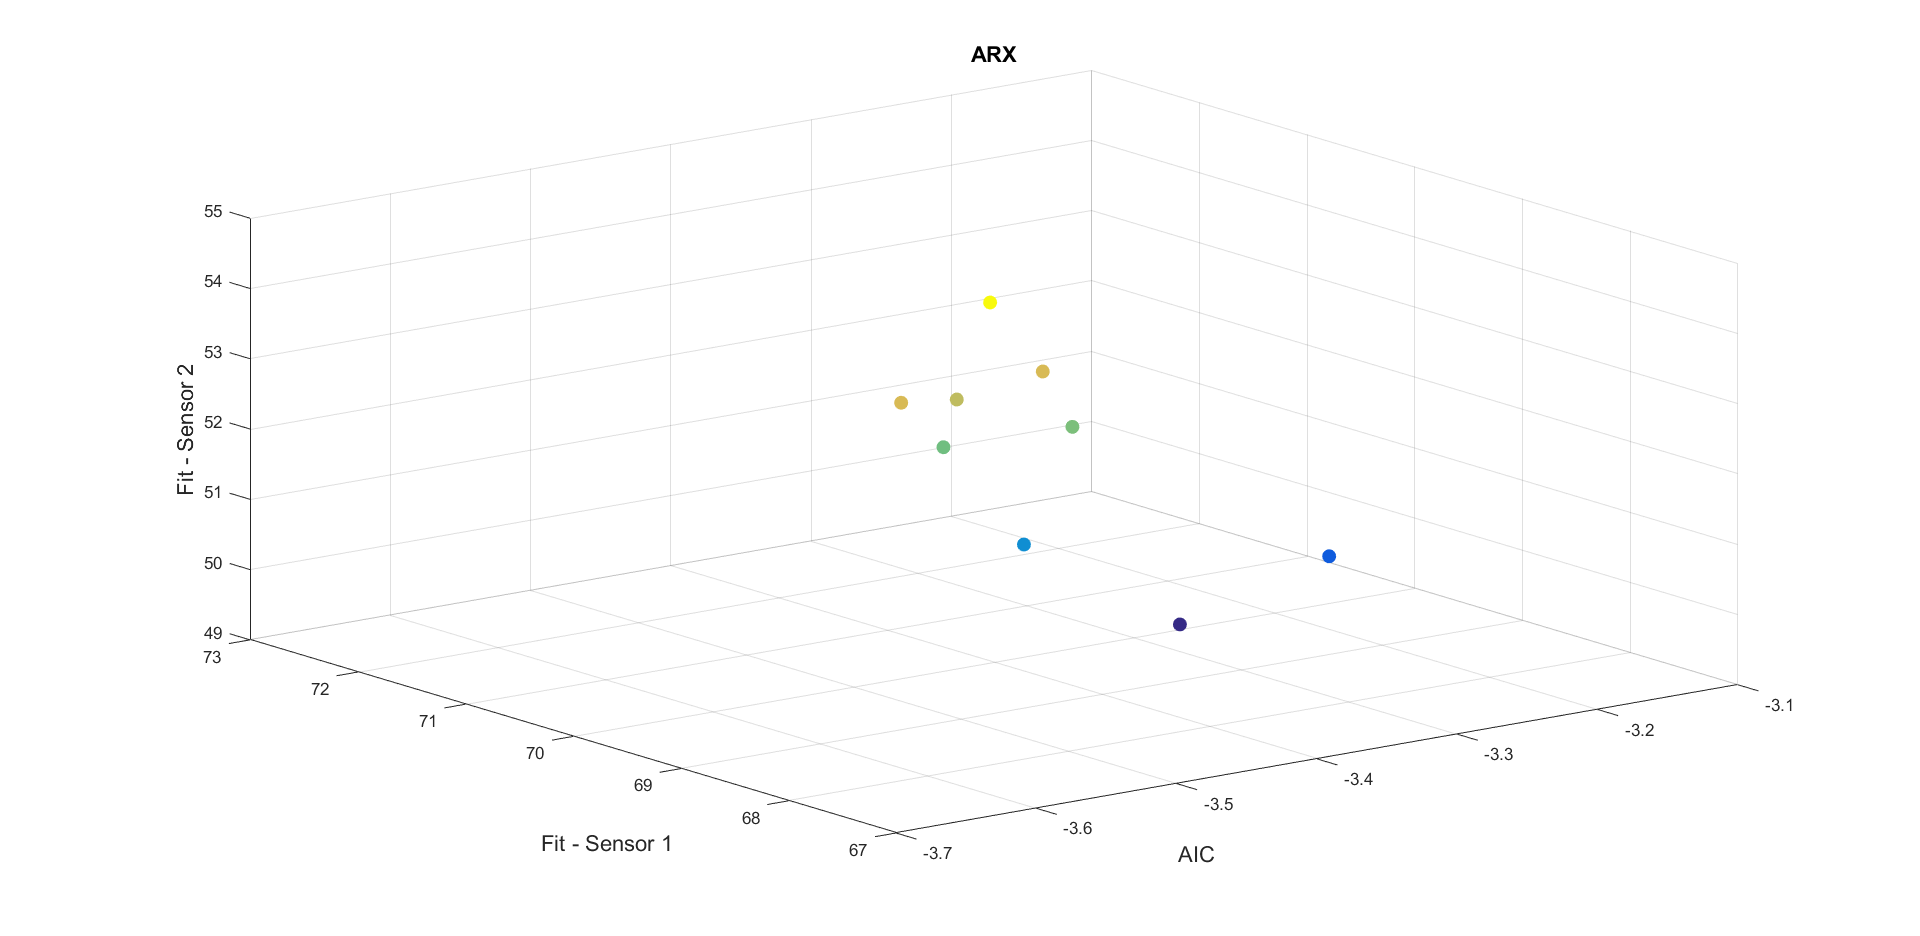
\includegraphics[width=1.00\textwidth]{./5_images/tclabsp-models-ARX.png} 
		\label{fig:tclabsp-models-arx}
	\end{center}
	\centering
	\makebox[\width]{Fonte: Autor} 
\end{figure}

\begin{table}[h]
	\centering
	\caption{Melhor modelo experimental - ARX}
	\label{tab:tclabsp-model-arx}
	\begin{tabular}{c|c} \toprule
		{Saída}			&	{Parâmetros}									\\ \midrule
		$Sensor_1$			&
								$ 
									\begin{aligned}
										\text{Formato:}																	\\
										A(z)y_1(t) &= - A_i(z)y_i(t) + B(z)u(t) + e_1(t)								\\
										\text{Onde:}																	\\
										A(z) &= 1 - 1.053 z^{-1} - 0.2885 z^{-2} + 0.4807 z^{-3} - 0.0593 z^{-4}		\\
										A_2(z) &= -0.1701 z^{-1} - 0.06197 z^{-2} + 0.1552 z^{-3} + 0.003291 z^{-4}		\\ 	 
										B1(z) &= 0.03937 + 0.04884 z^{-1} - 0.01257 z^{-2} - 0.02444 z^{-3}				\\	 
										B2(z) &= 0.005292 - 0.006813 z^{-1} - 0.005269 z^{-2} - 0.01209 z^{-3}   
									\end{aligned}
								$	
							\\ \midrule
		$Sensor_2$			&
								$ 
									\begin{aligned}
										\text{Formato:}																	\\
										A(z)y_2(t) &= - A_i(z)y_i(t) + B(z)u(t) + e_2(t)									\\
										\text{Onde:}																	\\
										A(z) &= 1 - 0.4421 z^{-1} - 0.3168 z^{-2} + 0.02046 z^{-3} - 0.02842 z^{-4}      \\ 
										A_1(z) &= -0.7006 z^{-1} + 0.02119 z^{-2} + 0.6253 z^{-3} - 0.1524 z^{-4}     	\\ 
										B1(z) &= 0.001822 - 0.02448 z^{-1} - 0.05453 z^{-2} - 0.03861 z^{-3}        	 	\\
										B2(z) &= 0.02737 + 0.03038 z^{-1} + 0.02127 z^{-2} + 0.01153 z^{-3}    			
									\end{aligned}
								$
							\\ \bottomrule
	\end{tabular}
	\caption*{Fonte: Autor}
\end{table}

\begin{figure}[h]
	\caption{Modelo: ARX - Teste de validação}
	\begin{center}
		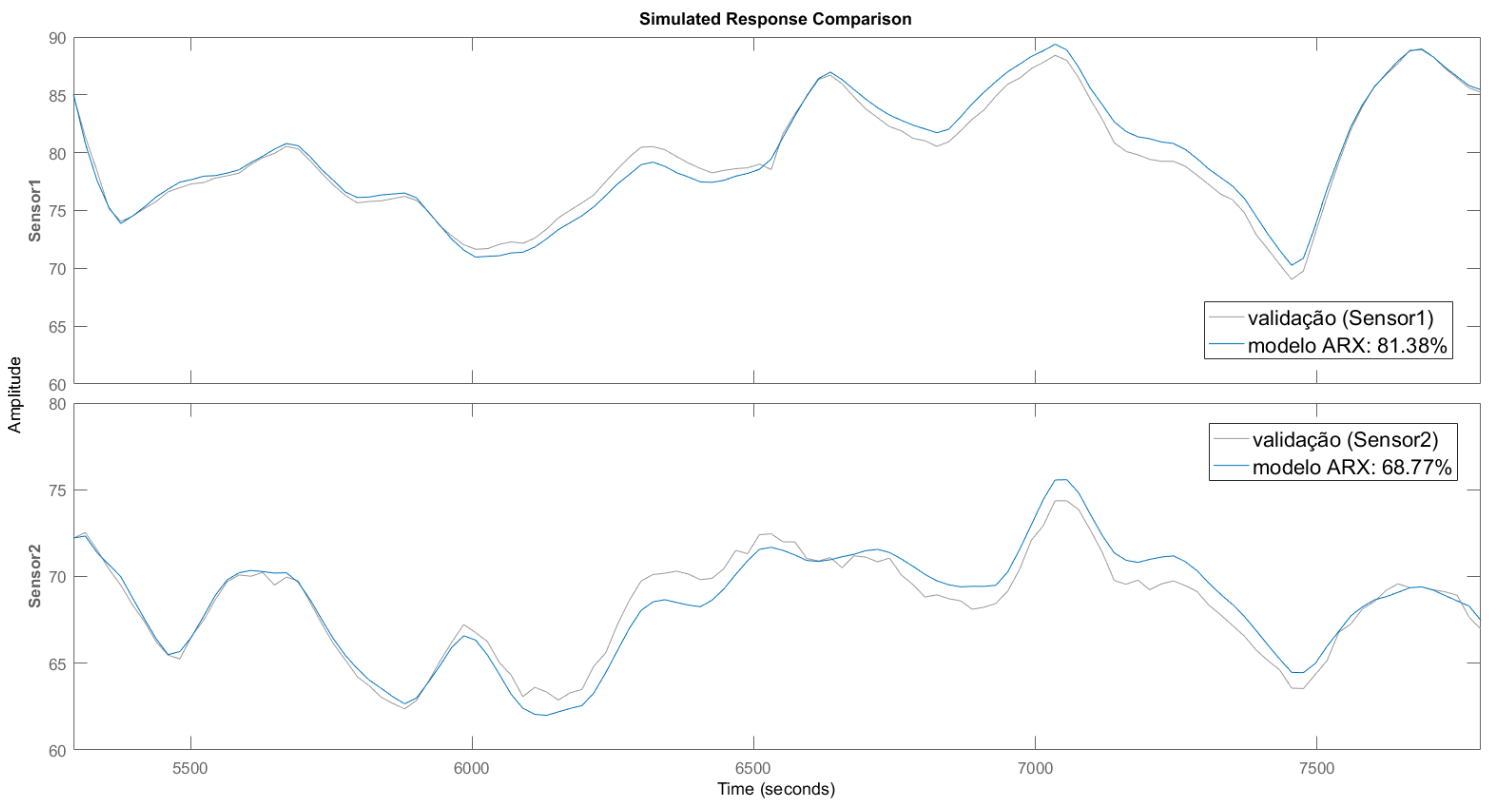
\includegraphics[width=1.00\textwidth]{./5_images/tclabsp-models-ARX-compare.png} 
		\label{fig:tclabsp-models-arx-compare}
	\end{center}
	\centering
	\makebox[\width]{Fonte: Autor} 
\end{figure}

\begin{figure}[h]
	\caption{Modelo: ARX - Análise de resíduos}
	\begin{center}
		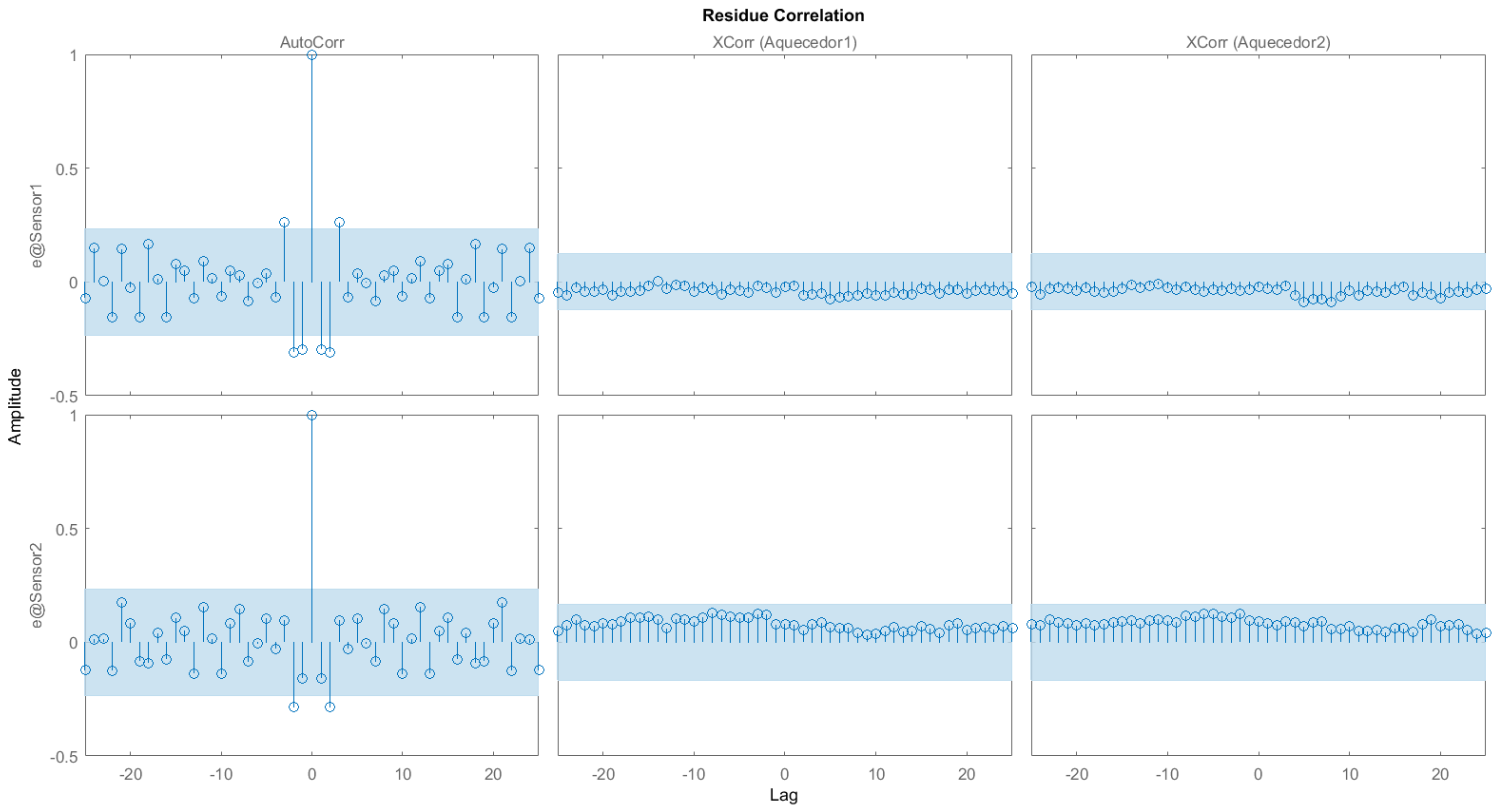
\includegraphics[width=1.00\textwidth]{./5_images/tclabsp-models-ARX-resid.png} 
		\label{fig:tclabsp-models-arx-resid}
	\end{center}
	\centering
	\makebox[\width]{Fonte: Autor} 
\end{figure}

% =====================================================================================================
% ============================================= Section ===============================================
% =====================================================================================================
\section{Desenvolvimento do controlador}
\label{sec:desenvolvimento_do_controlador}

Através das \cref{eq:tclab_modelo_siso,eq:tclab_modelo_mimo_a,eq:tclab_modelo_mimo_b}
e também do modelo experimental que será obtido da planta piloto, utilizaremos a representação de
espaço de estados para a construção do modelo que irá compor os controladores.

Serão utilizadas duas abordagens principais:

\begin{itemize}
    \item \textbf{Utilização apenas de linguagens de programação, sem o auxílio de ferramentas de desenvolvimento
        \acrshort{mpc}}: esta abordagem tem como meta aplicar o controle \acrshort{mpc} através dos algoritmos
        descritos nas obras de \citeonline{Wang2009}, \citeonline{Rawlings2015}, \citeonline{Rossiter2003},
        entre outros, com a finalidade de detalhar cada etapa dos cálculos realizados pelo controlador
        visando cumprir os seguintes objetivos descritos na seção \ref{sec:objetivos}: estudo do algoritmo do
        controle \acrshort{mpc}; comparação entre a implementação em duas ou mais plataformas e compilação
        de material teórico e experimental sobre \acrshort{mpc}.
    \item \textbf{Utilização de ferramentas de desenvolvimento \acrshort{mpc}}: esta abordagem visa utilizar
        ferramentas consolidadas de mercado para o desenvolvimento de controlador \acrshort{mpc}, como o
        \textit{Model Predictive Control Toolbox}, disponível no \acrshort{matlab} para poder realizar
        a comparação entre o desempenho de um controlador \acrshort{mpc} em comparação a um controlador
        \acrshort{pid}, como também foi proposto nos objetivos da seção \ref{sec:objetivos}.
\end{itemize}